\chapter{Desarrollo del Detector de Rostros y la Arquitectura de Red Neuronal Convolucional}

\section{Detección de Rostros}
En este trabajo se optó por utilizar como etapa inicial dentro de la fase de consultas a la red, la construcción de un detector de rostros, debido a que, al momento de desarrollar una aplicación orientada a las necesidades del mundo real, este no solo recibira como entrada imágenes que contengan exactamente el rostro de la persona, sino, imágenes con el cuerpo completo o algunas partes adicionales aparte del rostro. Sin embargo, en objetivo del trabajo es poder detectar la expresión facial de una persona, para lo cual, basta con tener como entrada a la red una imagen que delimite el rostro de la persona. De ahí, la necesidad de utilizar un algoritmo de detección de rostros para la extracción de la región de interes que posteriormente servira como entrada para la red neuronal convolucional encargada de reconocer la expresión facial correspondiente. La figura~\ref{fig:imagen_entrada} muestra un ejemplo de una imagen de entrada, en la cual, se puede observar detalles adicionales aparte del rostro (el sombrero y el fondo), los cuales no aportan carasterísticas relevantes que ayuden al reconocimiento de la expresión facial.

Para esta etapa se utilizó el detector de objetos \textit{haar cascade}, un algoritmo muy utilizado, cuya implementación puede ser encontrado en distintas librerías orientadas al procesamiento de imágenes, tales como OpenCV\footnote[5]{OpenCV es una librería \textit{open source} que contiene algoritmo relacionados con el area de visión por computador, http://opencv.org/}. Como se describió en la sección~\ref{sec:Haar_Cascade}, este algoritmo utiliza técnicas de \textit{machine learning}. Su proceso de entrenamiento se realiza con imágenes positivas y negativas (imágenes que representan y no representan rostros), creando así un modelo capaz de detectar rostros, basandose en la detección de características \textit{haar}. La entrada para esta etapa es una imagen cualquiera, el proceso consiste en detectar el rostro en dicha imagen (en caso exista algun rostro) y extraerlo en otra imagen en escala de grises, la cual tendra un tamaño aproximado de 48x48 píxeles (dependiendo de las dimensiones del rostro). Esta última imagen será la entrada para el modelo en la fase de consultas. Nótese que para la detección de un rostro y la asignación de su respectiva expresión facial, no es necesario mantener la imagen a color, puesto que este no es una característica necesaria para conseguir el objetivo. La figura~\ref{fig:proceso_deteccion} muestra los pasos a seguir para la detección y extracción del rostro en una imagen.

\begin{figure}[H]
		\centering
		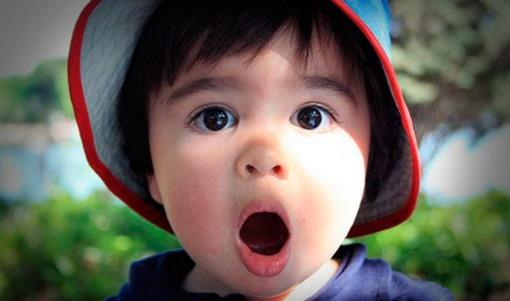
\includegraphics[width=50mm]{Imagenes/imagen_entrada.png}
		\caption{Ejemplo de una imagen de entrada.}
		\vspace{0.15cm}
		\textit{Fuente: Consuelo Ferrús, http://www.acompasando.org/orar-el-asombro/}
		\label{fig:imagen_entrada}
\end{figure}


\begin{figure}[H]
		\centering
		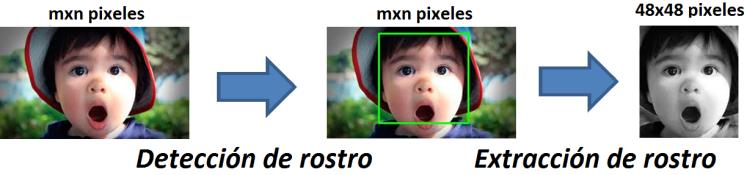
\includegraphics[width=140mm]{Imagenes/proceso_deteccion.png}
		\caption{Proceso de detección de rostro.}
		\vspace{0.15cm}
		\textit{Fuente: Propio}
		\label{fig:proceso_deteccion}
\end{figure}

Se optó por la utilización del detector de rostros \textit{haar cascade}, debido a que este es ampliamente utilizado por el nivel de precisión que posee~\cite{6russakovsky2015imagenet}. Sin embargo, esta técnica aun presenta algunas fallas cuando el rostro presenta algún tipo de oclusión (figura~\ref{fig:oclussion}). Este tipo de problema también puede ser solucionado construyendo una red convolucional orientada a la detección o localización de rostros, o por medio de otro tipo de técnicas tradicionales basadas en la extracción de características. Debido al tiempo y bajos recursos computacionales, se optó por proponer este tipo de enfoques como trabajos futuros.

\begin{figure}[H]
		\centering
		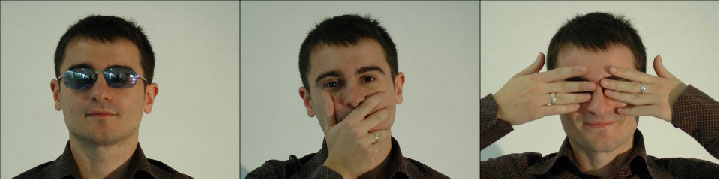
\includegraphics[width=130mm]{Imagenes/oclussion.jpeg}
		\caption{Ejemplo de rostros con oclusión.}
		\vspace{0.15cm}
		\textit{Fuente: Face Dataset, Universidad Politécnica de Catalunya.}
		\label{fig:oclussion}
\end{figure}

\section{Experimentación en la Elección de Parámetros y Capas en la Construcción de la Arquitectura CNN}
\label{sec:experiment}
La creación de un modelo robusto a partir de la utilización de redes neuronales convolucionales, es una tarea muy complicada, debido a que en la actualidad no existen estudios que indique cual es la configuración correcta que esta debe seguir. Es así, que todos los trabajos que utilizan cualquier técnica perteneciente a \textit{deep learning}, se basan en la experimentación sobre diversar configuraciones en la arquitectura, estas configuraciones estan relacionadas con el número de capas de convolución, sub-muestreo, totalmente conectadas, tipos de funciones de activacion y normalización. Otros elementos muy importantes que tambien son considerados al momento de realizar experimentos, son los parámetros de cada capa, tales como: el número y tamaño de los filtros en la capa de convolución, operaciones de agrupación en la capa de sub-muestreo, etc.

Sin embargo, entrenar un red neuronal no es una tarea fácil, debido a que se tienen que optimizar miles de parámetros para la creación de un buen modelo, asi como las miles de multiplicaciones de matrices que tienen que llevarse a cabo para realizar la operación de convolución. Es así que el número de experimentos que se puedan realizar, depende mucho de la insfraestructura y \textit{hardware} sobre el cual se esta trabajando, siendo este una gran limitante para una extensa experimentación.

Según lo explicado en los parrafos anteriores, para encontrar la correcta configuracion de una arquitectura basada en las redes neuronales convolucionales que resuelva el problema de reconocimiento de expresiones faciales, se realizaron muchos experimentos, cada uno con una configuracion diferente que la anterior. En total se evaluaron 3 arquitecturas con distintas configuracion de capas y parametros, en cada una de estas se calculo la precisión y error utilizando las bases de datos FER2013 y CK.




\begin{itemize}
\item {\textbf{Conv-Conv-Pool-Conv-Conv-Pool-FC}

\begin{table}[H]
    \centering
    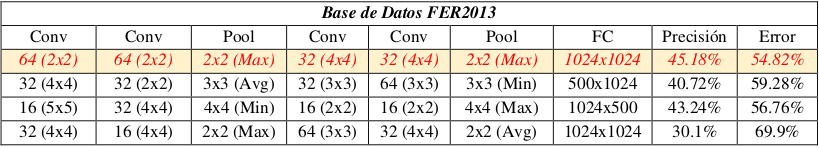
\includegraphics[width=140mm]{Imagenes/tabla_arqui_1_fer.png} 
    \caption{Evaluación de la arquitectura 1 y sus parámetros, FER2013}
    \label{tab:tabla_arqui_1_fer}
\end{table}

\begin{table}[H]
    \centering
    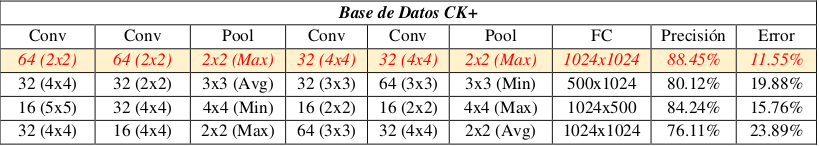
\includegraphics[width=140mm]{Imagenes/tabla_arqui_1_CK.png}
    \caption{Evaluación de la arquitectura 1 y sus parámetros, CK+}
    \label{tab:tabla_arqui_1_CK}
\end{table}

}

\item {\textbf{Conv-Pool-Conv-Pool-FC \underline{\textit{Arquitectura Propuesta}} }

\begin{table}[H]
    \centering
    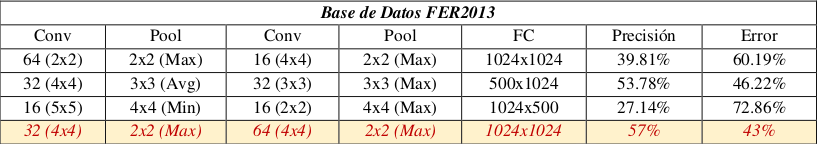
\includegraphics[width=140mm]{Imagenes/tabla_arqui_2_fer.png} 
    \caption{Evaluación de la arquitectura 2 y sus parámetros, FER2013}
    \label{tab:tabla_arqui_2_fer}
\end{table}

\begin{table}[H]
    \centering
    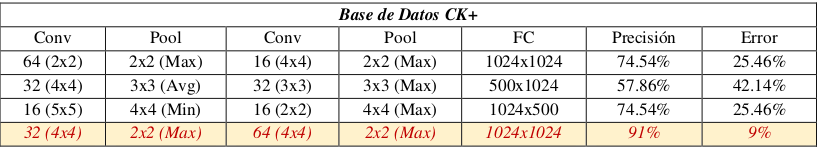
\includegraphics[width=140mm]{Imagenes/tabla_arqui_2_CK.png}
    \caption{Evaluación de la arquitectura 2 y sus parámetros, CK+}
    \label{tab:tabla_arqui_2_CK}
\end{table}

}

\item {\textbf{Conv-Pool-Pool-Conv-Conv-Pool-FC}

\begin{table}[H]
    \centering
    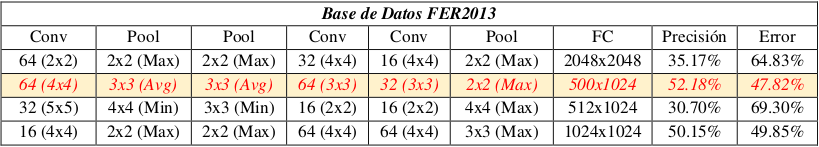
\includegraphics[width=140mm]{Imagenes/tabla_arqui_3_fer.png} 
    \caption{Evaluación de la arquitectura 3 y sus parámetros, FER2013}
    \label{tab:tabla_arqui_3_fer}
\end{table}

\begin{table}[H]
    \centering
    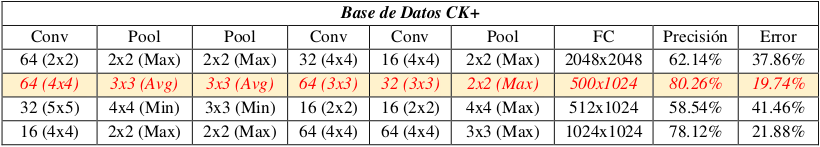
\includegraphics[width=140mm]{Imagenes/tabla_arqui_3_CK.png}
    \caption{Evaluación de la arquitectura 3 y sus parámetros, CK+}
    \label{tab:tabla_arqui_3_CK}
\end{table}
}
\end{itemize}

De acuerdo con los experimentos realizados, se puede obsevar que la mejor configuración de capas es: convolución-\textit{pooling}-convolución-\textit{pooling}-FC, con 32 y 64 filtros de tamaño 4$\times$4 en la primera y segunda capa de convolución respectivamente, ventanas de agrupación de 2$\times$2 en las dos capas de sub-muestreo y un total de 1024$\times$1024 neuronas en las últimas capas totalmente conectadas.

Según los resultados mostrados en las tablas~\ref{tab:tabla_arqui_1_fer} y~\ref{tab:tabla_arqui_1_CK} se puede concluir que, la utilización de dos capas consecutivas de convolución es una mala elección, debido a que el hecho de aplicar dos filtros consecutivos hace que la información de la imagen se pierda mas rápidamente que lo normal, ya que el tamaño de la imagen se reduce significativamente después de cada una de estas operaciones. También, las tablas~\ref{tab:tabla_arqui_3_fer} y~\ref{tab:tabla_arqui_3_CK} muestran resultados muy por debajo de la segunda configuración (la mejor obtenida en los experimentos realizados), similar que la explicacion anterior, se concluye que se dan estos resultados debido a la utilización de dos capas consecutivas de sub-muestreo, ya que el objetivo de estas capaz es reducir las dimensiones de la imagen solo preservando información relevante, sin embargo, al realizar una operación de sub-muestreo detras de otra, hace que se pierda más información de la necesaria. 

\section{Arquitectura Propuesta}
\label{sec:arq_propuesta}
De acuerdo con los experimentados mostrados en la sección~\ref{sec:experiment}, la arquitectura que consiguió los mejores resultados sigue la siguiente configuración: la entrada consta de una imagen de 48x48 píxeles en escala de gris, que es el resultado de la fase de detección y extracción de rostro, seguido de una capa de 32 convoluciones con filtro de 4x4 sin solapamiento, luego se aplica un sub muestreo de 2x2 con función MAX \footnote[6]{Función que determina el máximo de n números.} , seguido de una capa de 64 convoluciones con filtros de 2x2 sin solapamiento, para posteriormente aplicar un sub muestreo también de dimensiones 2x2 con función MAX, aplicada las convoluciones y sub muestreo se procede a aplicar el Dropout\footnote[7]{Una forma simple de prevenir el \textit{overfitting} en redes neuronales.} con 20\%, seguido de dos capas, con 1024 neuronas totalmente conectadas cada una. Finalmente, para la clasificación se aplica la función de normalización Softmax, la cual toma 6 clases, las cuales representar al número de expresiones a reconocer.
\vspace{0.5cm}
\begin{table}[H]
    \centering
    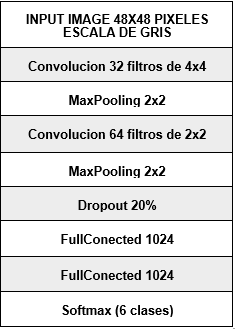
\includegraphics[width=60mm]{Imagenes/tabla_arquitectura.png}
    \caption{Arquitectura del modelo propuesto}
    \label{tab:tabla_arquitectura}
\end{table}


\begin{figure}[H]
		\centering
		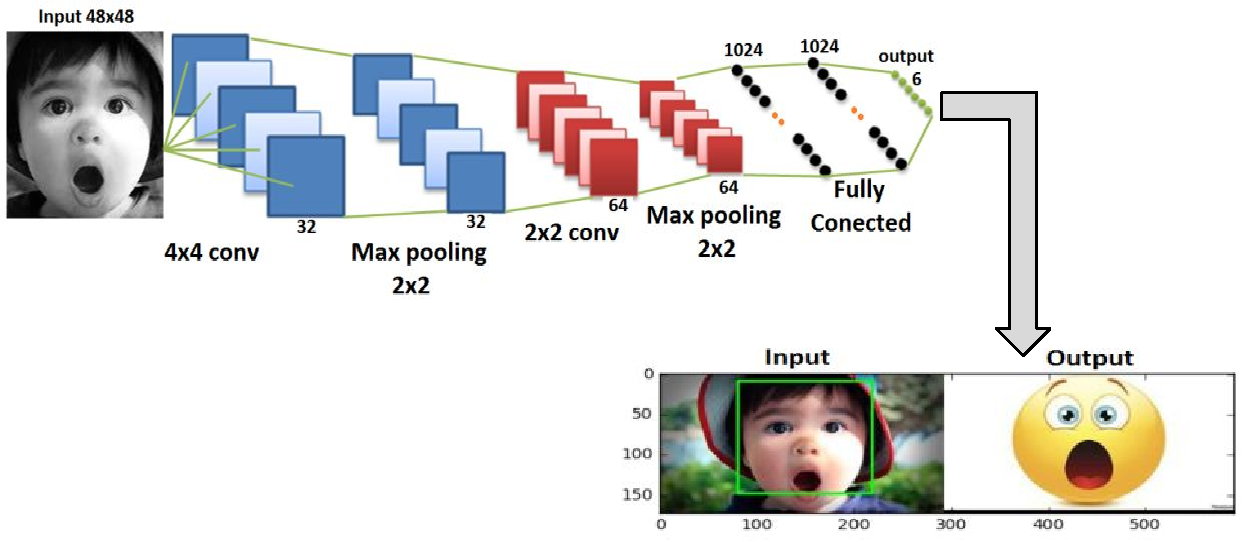
\includegraphics[width=180mm]{Imagenes/arquitectura_CNN_grafico.pdf}
		\caption{Arquitectura gráfica del modelo propuesto.}
		\vspace{0.15cm}
		\textit{Fuente: Propio.}
		\label{fig:arquitectura_CNN_grafico}
\end{figure}

La tabla~\ref{tab:tabla_arquitectura} muestra de arriba para abajo, la representación secuencial de las capas dentro de la arquitectura propuesta antes mencionada. Sin embargo, La figura~\ref{fig:arquitectura_CNN_grafico} muestra de una forma mas detallada cada una de las capas que integran la arquitectura, construyendo de esta forma una red neuronal convolucional. También se muestra en esta figura, la salida final obtenida despues de realizar una consulta sobre el modelo, resaltando el rostro detectado en la imagen de entrada, y relacionando la expresión facial que este tiene con una imagen caricaturizada. El código fuente y los conjuntos de datos estan disponibilizados en
\href{https://github.com/CodeBlueDS/Code---Facial-expression-recognition-}{link 1} y \href{https://drive.google.com/drive/folders/1vMJIC8TW1NX7ffMbyZPraySLGV6hnGK7?usp=sharing}{link 2} respectivamente.

\section{Descripción de la Capas de la Arquitectura}

Dentro de cada capa perteneciente a la red neuronal convolucional, se lleva a cabo operaciones de multiplicación de matrices, agrupación de regiones, etc, con el objetivo de extraer o resaltar características importantes de las cuales la red pueda aprender patrones y filtros que se adapten mejor al problema, de tal forma que pueda dar respuestas precisas a entradas futuras. 

Siguiendo el orden de capas de la arquitectura propuestas, presentada en la sección~\ref{sec:arq_propuesta}, se describe el comportamiento de cada uno de ellos de la siguiente forma: 
\begin{itemize}
\item
{
\textbf{Primera capa convolución.} Cuenta con 32 filtros (mapa de características) de tamaño 4x4 píxeles. Esta capa tiene como objetivo extraer características de alto nivel. La figura~\ref{fig:filtro1} muestra el conjunto de imágenes generadas después de aplicar los 32 filtros de convolución sobre la imagen de entrada, estas imágenes muestra claramente que en esta capa, la arquitectura se encarga de aprender filtros que sean capaces de extraer bordes y partes fundamentales del rostro, tales como: los ojos, boca, nariz y cejas. Esta primera capa de convolución genera una imagen de salida por cada filtro, siendo así, 32 nuevas imágenes las entradas para la siguiente capa. 

\begin{figure}[H]
		\centering
		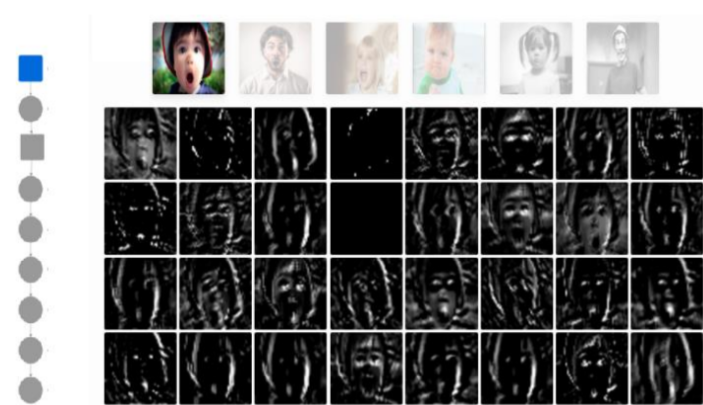
\includegraphics[width=100mm]{Imagenes/filtro1.png}
		\caption{Imágenes de salida después de la primera convolución.}
		\vspace{0.15cm}
		\textit{Fuente: Propio.}
		\label{fig:filtro1}
\end{figure}
}

\item
{
\textbf{Primera capa de \textit{pooling} o sub-muestreo.} Recibe como parámetros de entrada, las 32 imágenes generadas a partir de la primera capa de convolución. Su función es la de reducir características redundantes mediante la agrupación de pixeles y eleccion del mejor de entre ellos, esta agrupacion se realiza en sub-regiones no solapadas de la matriz, de dimensiones 2$\times$2. Despues de obtener estas sub-regiones, se obtiene el máximo pixel de entre ellas para ser la salida de dicha sub-región. La figura~\ref{fig:filtro2} muestra imágenes semejantes a las obtenidas por la primera capa de convolución, esto se debe a que esta capa no realiza ninguna alteración en el valor de los píxeles, mas al contrario, esta encargada de reducir las dimensiones de las imágenes de entrada, eliminando los píxeles menos significativos. Debido a que se aplica este tipo de operaciones a cada imagen de entrada de esta capa, su número de imágenes de salida sera igual a su número de entradas.

\begin{figure}[H]
		\centering
		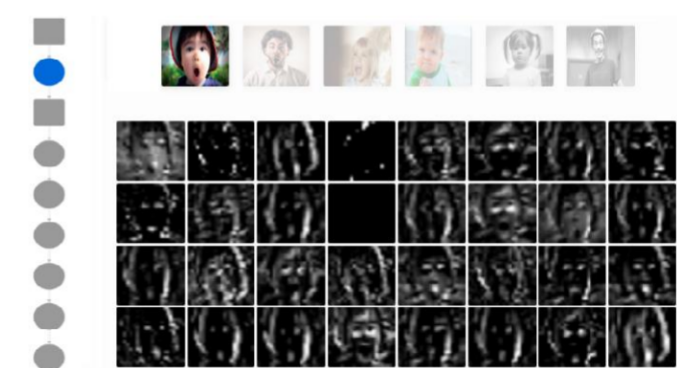
\includegraphics[width=100mm]{Imagenes/filtro2.png}
		\caption{Imágenes de salida después del primer sub-muestreo.}
		\vspace{0.15cm}
		\textit{Fuente: Propio.}
		\label{fig:filtro2}
\end{figure}
}

\item
{
\textbf{Segunda capa de convolución.} Cuenta con 64 filtros y recibe como parámetros de entrada las imágenes generadas a partir de la primera capa de sub-muestreo. A diferencia de la primera capa de convolución, su función es la de extraer y detectar características de más bajo nivel. La figura~\ref{fig:filtro3} muestra las 64 imágenes generadas a partir los filtros de esta capa, en ellas se puede observar de manera más abstracta ciertos puntos y rectas que representan partes del rostro de la imagen de entrada. Como se menciono anteriormente, esta capa origina 64 imágenes de salida, cada una con un tamaño de 21$\times$21 píxeles.

\begin{figure}[H]
		\centering
		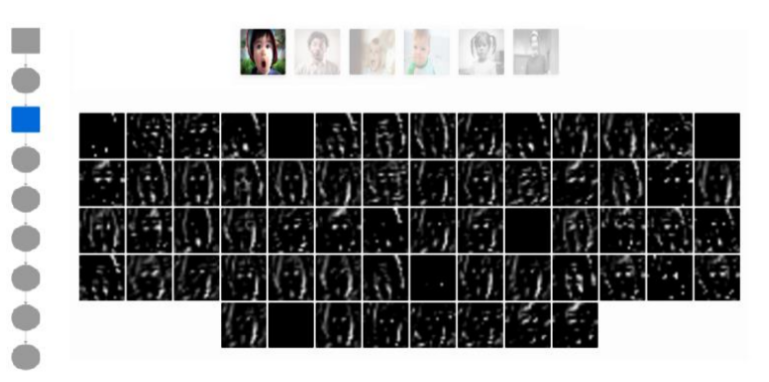
\includegraphics[width=100mm]{Imagenes/filtro3.png}
		\caption{Imágenes de salida después de la segunda convolución.}
		\vspace{0.15cm}
		\textit{Fuente: Propio.}
		\label{fig:filtro3}
\end{figure}
}

\item
{
\textbf{Segunda capa de \textit{pooling} o sub-muestreo.} Recibe como parámetros de entrada las imágenes generadas a partir de la segunda capa de convolución. Similar que la primera capa de sub-muestreo, es la encargada de eliminar características no relevantes de las imágenes de entrada, mediante la agrupación y selección del mejor pixel, las sub-regiones de agrupación son de dimensiones 2$\times$2. La figura~\ref{fig:filtro4} muestra las 64 imágenes generadas a partir de esta capa, donde cada una de estas nuevas imágenes son de tamaño 10x10 píxeles. Segun esta figura se puede observar que el rostro se distorsiona y pierde su forma original, siendo estas, a lo que se conoce como características de bajo nivel.
\begin{figure}[H]
		\centering
		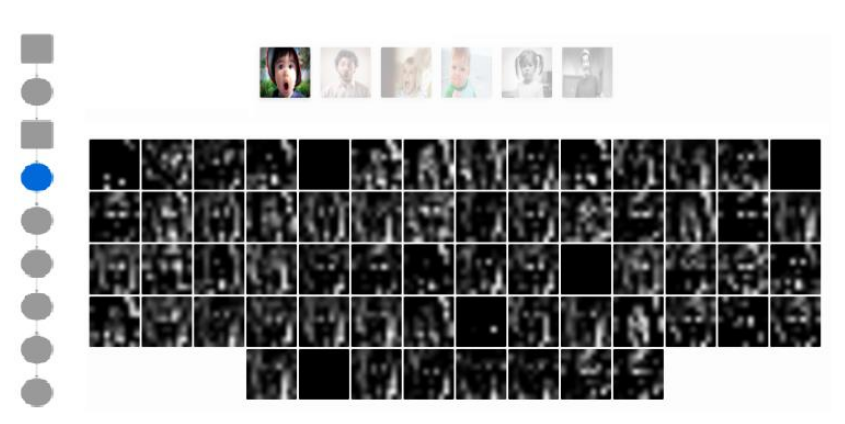
\includegraphics[width=100mm]{Imagenes/filtro4.png}
		\caption{Imágenes de salida después del segundo sub-muestreo.}
		\vspace{0.15cm}
		\textit{Fuente: Propio.}
		\label{fig:filtro4}
\end{figure}
}
\item
{
\textbf{Capas totalmente conectadas.} Recibe como parámetros de entrada las imágenes generadas a partir de la segunda capa de sub-muestreo, las cuales representan las características a bajo nivel pertenecientes a la imagen de entrada original. El objetivo de esta capa, es relacionar cada una de estas características por medio de las 2 capas totalmente conectadas con 1024 neuronas cada una, donde cada neurona es una imagen que representa alguna característica encontrada en las capas anteriores. Al final de la arquitectura, se utiliza la función de normalización \textit{softmax} para generar 6 salidas, donde cada una de ellas representa a una expresión facial. La función de normalización es la encargada de asignar una probabilidad a cada una de estas salidas, siendo nuestra salida final, aquella que presente la mayor probabilidad.
}
\end{itemize}

\section{Parámetros de la Arquitectura}

El número de parámetros que contiene una determinada arquitectura, depende mucho del número de capas, filtros, y neuronas en la capa totalmente conectada. Conocer la cantidad de parámetros en una red, es de gran utilidad, debido a que gracias a ellos podemos hacernos una idea de cuan difícil o fácil es entrenar esta. Por tanto, mientras una red o arquitectura tenga mas parámetros, esta será más costosa, obviamente, debido a la gran cantidad de parámetros por optimizar. Sin embargo, la cantidad de parámetros no necesariamente refleja la robustés de una red para una determinada tarea. Por ejemplo, puede existir problemas que con pocos parámetros a optimizar sean mejores que considerando complejas arquitecturas, o de forma viceversa.

Una manera más fácil de entender el comportamiento de la optimización de parámetros, es ver esta red como una función, donde, las salidas o etiquetas de cada entrada son el resultado de la función y cada variables son las entradas, siendo el principal objetivo, optimizar todas las constantes que multiplican a las variables, de tal manera que la función se ajuste para todas las entradas y de las salidas correctas. 

La tabla~\ref{tab:parametros} muestra la cantidad de parámetros obtenidos por la red. Un detalle muy importante, es que la capas de sub-muestreo no contienen ningún tipo de párametro a optimizar, esto es debido a que la función de agrupación es fija y no necesita ser modificada. Sin embargo, en la capa de convolución los filtros inicialmente son ceros, y son modificados en cada etapa de entrenamiento, lo mismo ocurre con las neuronas de las últimas capas totalmente conectadas. La cantidad total de parámetros es 7,620,199, distribuídos de la siguiente forma: 

\begin{itemize}
\item Primera capa con 32 convoluciones: 544 parámetros
\item Segunda capa con 64 convoluciones: 8256 parámetros
\item Primera capa totalmente conectada: 6554624 parámetros
\item Segunda capa totalmente conectada: 1049600 parámetros
\item función de normalización Softmax: 7175 parámetros
\end{itemize}

\begin{table}[H]
    \centering
    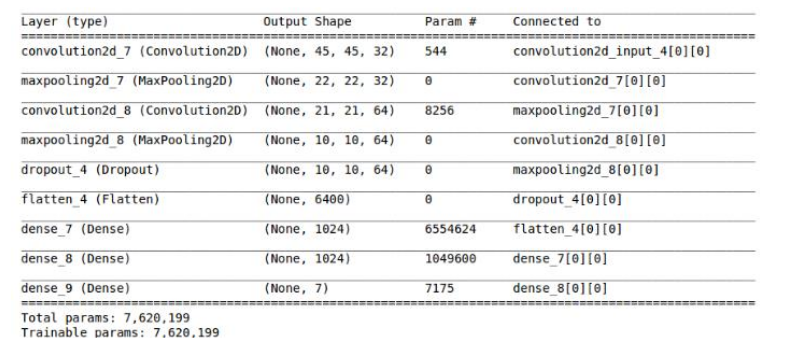
\includegraphics[width=160mm]{Imagenes/parametros.png} 
    \caption{Número de parámetros de la arquitectura propuesta.}
    \label{tab:parametros}
\end{table}

	
\section{Entrenamiento de la Red}

Se abordo esta tarea como un problema de aprendizaje supervisado. Como se relato en la sección~\ref{sec:deep-learning}, este tipo de aprendizaje requiere como datos de entrada, imágenes con una respectiva etiqueta, la cual indica la expresión facial a la que representa dicha entrada. Por lo tanto, descrito de una manera muy superficial y general, el proceso de entrenamiento consiste en ingresar imágenes de entradas con sus respectivas etiquetas a la red e intentar que esta aprenda a modelar sus pesos de tal manera que alcance las salidas deseadas. Este proceso se realiza con la ayuda del algoritmo de aprendizaje \textit{backpropagation}, el cual propaga el error final obtenido hacia las neuronas de las capas anteriores que colaboraron en la obtención de dicho resultado.

Como se mencionó en el anterior párrafo, la etapa de entrenamiento consiste en ingresar todos los datos y esperar que la red aprenda de ellos por medio de algoritmos de aprendizaje. Sin embargo, generalemente nunca es suficiente una sola iteración de este proceso, por lo que, se repite dicho proceso $x$ veces, siendo $x$ mas conocido como el número de \textit{épocas}. Debido a que este tipo de algoritmos son basados en prueba y error, el entrenamiento se realiza hasta que la red comience a dar señales de sobreajuste de pesos, es decir, el aprendizaje ya no mejora, mas bien empeora. En conclusión, los resultados no necesariamente serán mejores mientras mas sea el número de épocas, como se menciono antes, este tipo de abordage(\textit{deep learning}) en la actualidad no tiene un estudio previo que indique la cantidad de parámetros, capas, épocas y funciones que una red deba tener, por lo tanto, la respuesta esta en la cantidad de experimentos que se realicen, pero debido al poder computacional y tiempo que este requiere, es una limitante para todos los investigadores en el mundo. 

Para los experimentos realizado en la fase de entrenamiento, orientados a resolver el problema planteado (reconocimiento de expresiones faciales), se siguieron los pasos antes descritos y se observó que después de la época 100 la red deja de aprender. Esta descripción se muestra de manera mas detallada (por cada base de datos experimentada) en la sección~\ref{sec:experiment}.

\section{Pruebas al Modelo Creado}

La fase de entrenamiento da origen a un archivo con extensión .h5, el cual almacena los pesos de la red. Ya con este archivo en mano, se realiza la siguiente etapa, que consiste en las pruebas al modelo creado. Estas pruebas o consultas siguen la siguiente secuencia de pasos: 

\begin{itemize}
\item Primero, se lee una imagen como dato de entrada, de dimensiones mayor o igual a 48x48 píxeles. La imagen puede ser a colores o no, el algoritmo internamente lo procesa como una imagen en escala de gris.
\item Segundo, para reducir la cantidad de información irrelevante en la imagen (partes de la imagen que no pertenecen a un rostro: cuerpo, fondo, etc), se utiliza el detector de rostros \textit{haar cascade}, obteniendo así, cuatro coordenadas que delimitan el rostro en la imagen de entrada.
\item Tercero, ya con las cuatro coordenadas obtenidas por el algoritmo de detección, se recorta la imagen. Si la imagen recortada resulta ser de tamaño menor que 48$\times$48 píxeles, esta se redimensiona a dicho tamaño. Caso contrario la imagen se mantiene tal cual.
\item Cuarto, la imagen obtenida en el paso anterior es pasada como dato de consulta al modelo. Este devuelve un valor entero en el intervalo $[0-6]$, donde cada uno de esos numeros representa una expresion facial. Finalmente, se muestra como imagen de salida la imagen de consulta con una figura caricaturizada que esta relacionada con el número obtenido.
\end{itemize}

La figura~\ref{fig:test} muestra los pasos 3 y 4 mencionadas en los párrafos anteriores.

\begin{figure}[H]
		\centering
		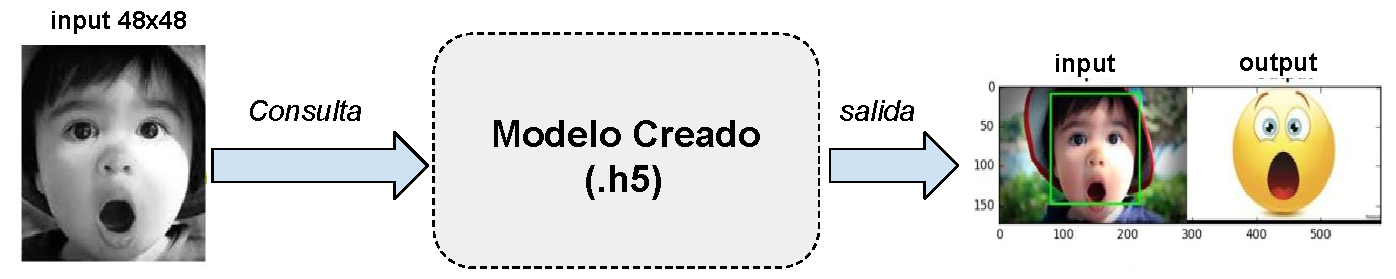
\includegraphics[width=160mm]{Imagenes/test.pdf}
		\caption{Secuencia de pasos en la fase de pruebas.}
		\vspace{0.15cm}
		\textit{Fuente: Propio.}
		\label{fig:test}
\end{figure}

\section{Recopilación de Imágenes de Expresiones Faciales.}
En la actualidada el internet nos ha abastecido con grandes cantidades de información. Dentro de estas, podemos encontrar comunidades dedicadas a la investigación que proveen bases de datos de imágenes etiquetadas relacionadas con problemas específicos, tales como: el reconocimiento de placas de automóviles, clasificación de imagenes o como en nuestro caso, reconocimiento de expresiones faciales. Estas bases de datos son utilizadas por toda la comunidad científica, publicando y comparando sus resultados con trabajos previos y acercandoce más y más a un margen de error mínimo. Generalemente estas bases de datos cuentan con imágenes cuidadosamente seleccionadas, intentando cubrir todos los casos posibles que se podrian presentar en escenas de la vida real. 

Como se mencionó en el párrafo anterior, en este trabajo, la recopilación de las imágenes de expresiones faciales se obtuvo de 2 fuentes secundarias de información (internet) en los cuales los datos están pre-elaborados. La primera base de datos utilizada es contiene imagenes de 48$\times$48 píxeles de tamaño, mientras que la segunda de 640$\times$480 o 640$\times$490 píxeles. Para la fase de prueba también se utilizaron imágenes aleatórias de internet, dentro de estas imágenes se consideran personas del mundo real y caricaturizadas (ver figura~\ref{fig:caricaturizado}).

\begin{figure}[H]
		\centering
		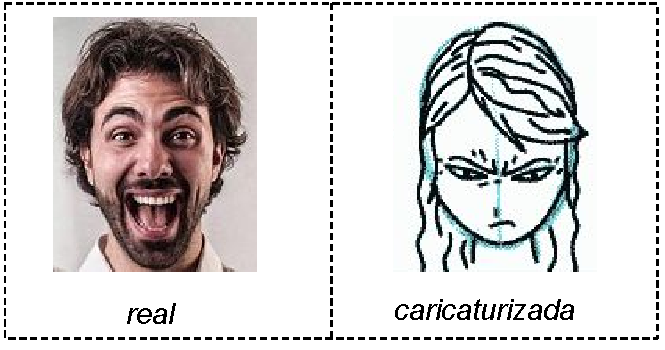
\includegraphics[width=110mm]{Imagenes/pruebas.pdf}
		\caption{Ejemplo de un rostro real y caricaturizado.}
		\vspace{0.15cm}
		\textit{Fuente: Internet.}
		\label{fig:caricaturizado}
\end{figure}

\section{Base de Datos}
Para la realización de experimentos se utilizaron 3 bases de datos, dos de ellas se encuentran disponibilizadas en internet(\textit{FER103} y \textit{CK+}) y una tercera que es resultado de la unión de estas dos anteriores. Se optó por considerar esta tercera base de datos, debido a que el abordage de \textit{deep learning} trabaja mejor mientras tenga mas datos para la fase de entrenamiento.
 
\subsection{FER2013}
\label{subsec:fer2013}
Es una base de datos del sitio web \textit{Kaggle}, destinada para el concurso de reconocimiento de expresiones faciales. Fue preparada por Pierre-Luc Carrier y Aaron Courville, como parte de un proyecto de investigación en curso. Esta clasificada en 7 categorías: molesto, disgustado, miedo, feliz, triste, sorpresa y neutro, sin embargo, en este trabajo se optó por unir la categoría enojado y disgustado debido a las similitudes que ambas tienen.

Este conjunto de datos está disponible como archivos \textit{train.csv} y \textit{test.csv}, los cuales contienen 2 columnas: \textit{emotion} y \textit{pixels}. La columna \textit{emotion} contiene un código numérico en el rango de 0 a 6 inclusive, para la expresión que esta presente en la imagen. La columna \textit{pixels} contiene un string de números que representa los valores para cada pixel dentro de la imagen. El conjunto de entrenamiento consiste de 28,709 ejemplos, mientras que los datos de prueba son 3589. La figura~\ref{fig:imagenes_fer} muestra ejemplos de imágenes de este conjunto de datos.


\begin{figure}[H]
		\centering
		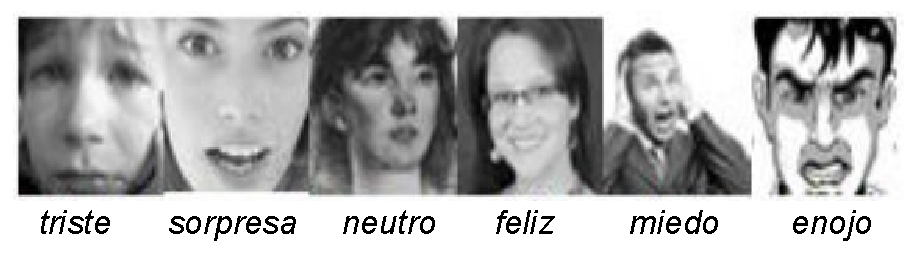
\includegraphics[width=110mm]{Imagenes/imagenes_fer.pdf}
		\caption{Imágenes de la base de datos FER2013}
		\vspace{0.15cm}
		\textit{Fuente: Kaggle.}
		\label{fig:imagenes_fer}
\end{figure}

\subsection{CK$+$}
\label{subsec:ck+}
La base de datos CK+ (Cohn-Kanade) posee imágenes de expresiones faciales frontales de 210 diferentes personas. Estas imágenes tienen una resolución original de 640x490 y 640x480 píxeles. Debido a que solo se encontraron imágenes pertenecientes a esta base de datos y sin ninguna etiqueta que relacione la expresión facial que representa cada una de ellas, en este trabajo se optó por realizar la etiquetación de forma manual (basandonos en el trabajo de Paul Ekman), obteniendo así 3289 imágenes, transformandolas a imágenes en escala de gris con dimensiones de 48x48 píxeles. Similar que la anterior base de datos, se consideraron 6 categorías (enojado, miedo, feliz, triste, sorprendido y neutro). Se utilizó el 80\% del total de imagenes para la fase de entrenamiento (2966 imágenes) y el 20\% para la fase de pruebas (323 imágenes). La figura~\ref{fig:imagenes_ck+} muestra ejemplos de imágenes de este conjunto de datos.

\begin{figure}[H]
		\centering
		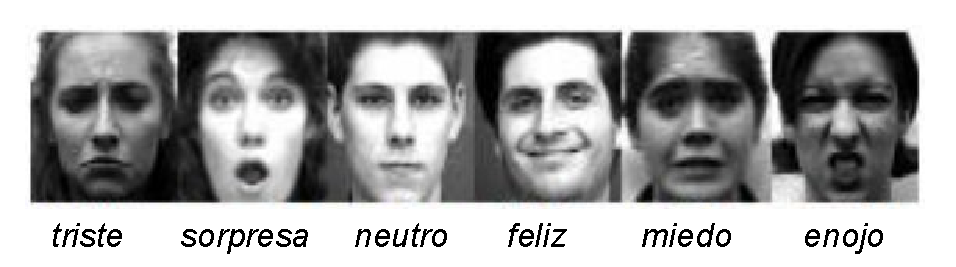
\includegraphics[width=110mm]{Imagenes/imagenes_ck+.pdf}
		\caption{Imágenes de la base de datos CK+}
		\vspace{0.15cm}
		\textit{Fuente: Base de datos CK+.}
		\label{fig:imagenes_ck+}
\end{figure}


\subsection{FER2013 - CK$+$}
\label{subsec:ck+fer2013}
Esta base de datos resulta de la unión de las dos anteriores (Fer2013 y CK+), obteniendo así un total de 39176 imágenes en escala de gris de dimensiones de 48x48 píxeles. El conjunto de entrenamiento es el 80\% del total (35264 imagenes), mientra que el conjunto de prueba es el 20\% (3912 imagenes). Se realizo esta unión de datos con la finalidad de obtener un modelo más robusto, ya que las técnicas de \textit{deep learning} dependen mucho de la cantidad de datos para el entrenamiento de un modelo.

\section{Resultados Experimentales}
\label{sec:experiment}

Los experimentos se realizaron sobre los tres conjuntos de datos mencionados en la sección anterior. En esta sección se muestran los resultados de dichos experimentos uno por uno, donde se podrán apreciar los niveles de precisión alcanzados por cada categoría - expresion facial, así como sus matrices de confusión, las cuales ayudan para un mejor entendimiento e interpretación de los resultados. También son mostrados por medio de gráfico, el aprendizaje de la red medido en términos de precisión durante cada época.

Para una mejor comprensión e interpretación de los resultados, se definen las siguiente palabras: \textit{precisión} es la fracción de instancias (datos de entrada) que alcanzaron un resultado correcto entre el número de instancias totales, \textit{recall} es la cantidad de intancias correctas recuperadas sobre la cantidad total de instancias relevantes (falsos positivos y falsos negativos). La figura~\ref{fig:precisionRecall} muestra de una manera mas sencilla ambas definiciones. Por otro lado \textit{f1-score} es la media armónica de la precisión y el \textit{recall}, la ecuación~\ref{eq:f1-score} muestra su representación matemática. \textit{Falsos positivos} o \textit{falses positives} en ingles, son el conjunto de instancias cuyas respuestas se creen que son correctas cuando en realidad estan erradas. \textit{Falsos negativos} o \textit{false negatives} a diferencia del anterior, son el conjunto de instancias que creen que estan errados cuando en realidad son correctos. \textit{verdaderos positivos} y \textit{verdaderos negativos} son simplemente instancias que son o bien correctas o erroneas.

\begin{figure}[H]
		\centering
		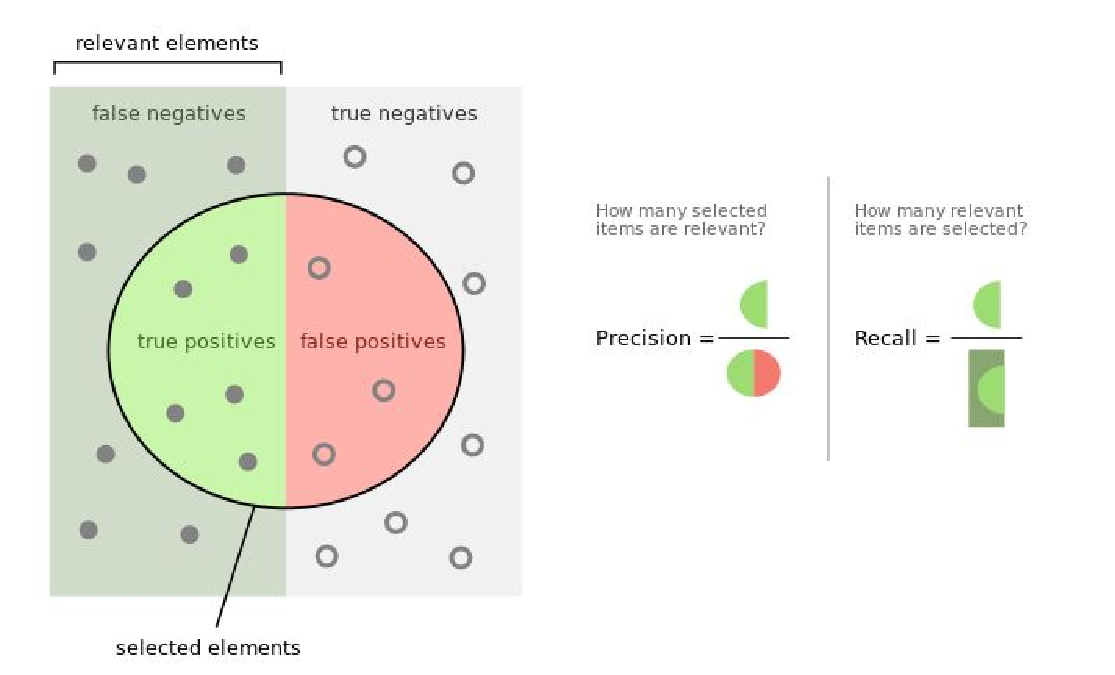
\includegraphics[width=120mm]{Imagenes/Precisionrecall.pdf}
		\caption{Precision y recall.}
		\vspace{0.15cm}
		\textit{Fuente: Precision and recall, Wikipedia.}
		\label{fig:precisionRecall}
\end{figure}

\begin{equation}\label{eq:f1-score}
F1 = 2\times\frac{precision\times recall}{precision + recall}
\end{equation}

\subsection{FER2013}

\begin{table}[H]
    \centering
    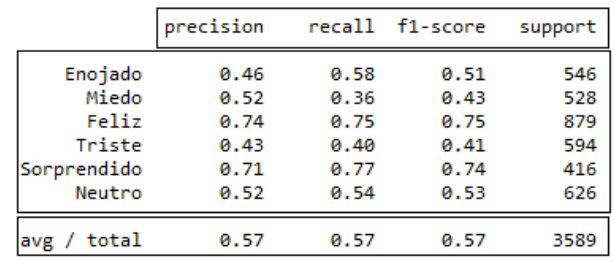
\includegraphics[width=100mm]{Imagenes/tabla_resultados_fer.png} 
    \caption{Resultados obtenidos - FER2013}
    \label{tab:tabla_resultados_fer}
\end{table}

En la tabla~\ref{tab:tabla_resultados_fer} se muestra los resultados obtenidos durante los experimentos realizados en la base de datos FER2013. Dentro de los niveles de precisión y \textit{recall}, se observa que las categorías 'feliz' y 'sorpresa' obtienen mejores resultados que las demás, alcanzando un nivel de precisión de 74\% y 71\% respectivamente. Por otro lado, la categoría 'enojado' alcanza 46\%, siendo la más baja de entre todas. El resultado general alcanzado en este conjunto de datos es de 57\%.

\begin{figure}[H]
		\centering
		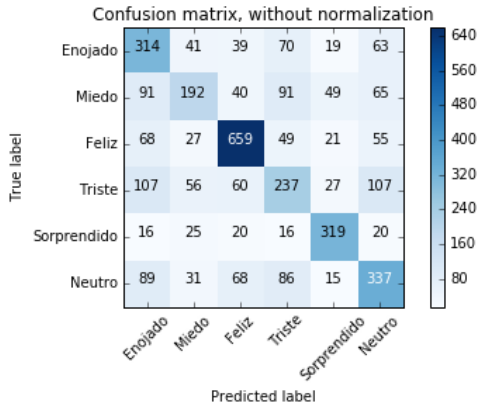
\includegraphics[width=90mm]{Imagenes/matriz_confusion_fer.png}
		\caption{Matriz de confusión, precisión del Test - FER2013}
		\label{fig:matriz_confusion_fer}
\end{figure}

Gracias a la matriz de confusión (figura~\ref{fig:matriz_confusion_fer}) se puede descubrir con exactitud la cantidad de datos que fallan y aciertan por categoría. Como se mencionó anteriormente, la categoría 'feliz' es la que presenta mayor precisión, acertando 659 imágenes de las 879 en total, también podemos observar que la red confunde esta categoría en mayor cantidad con la categoría 'neutro', siendo en total 68 imágenes de expresiones faciales 'neutras' confundidas con expresiones de la categoría 'feliz'. Otro detalle muy importante que nos muestra esta imagen, es que la red confunde en grandes cantidades las categorías 'triste' con 'enojado' y 'neutro', lo que nos da a entender que deberiamos poner mas enfasis e importancia en imágenes pertenecientes a estas categorías.  
\begin{figure}[H]
		\centering
		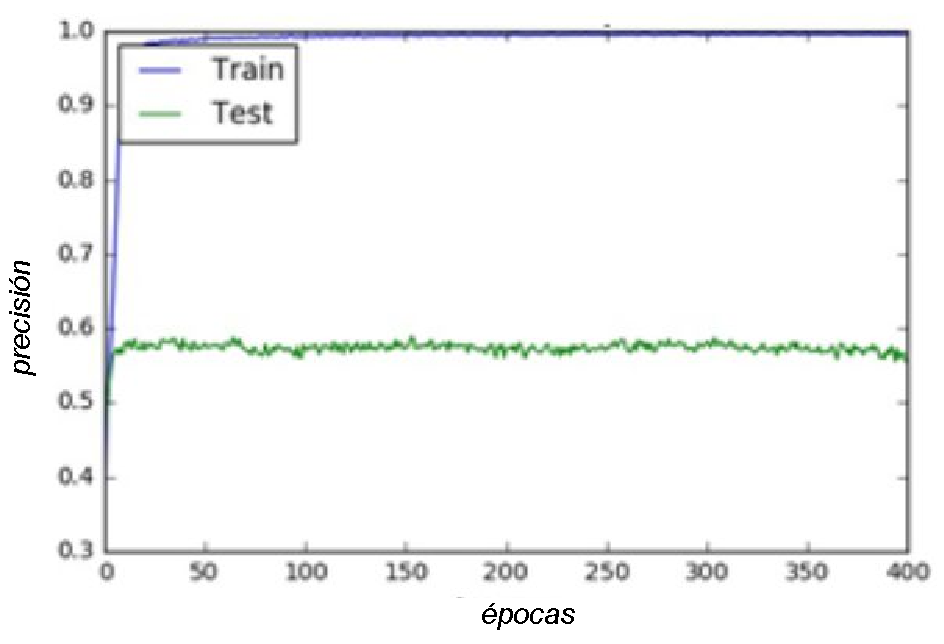
\includegraphics[width=95mm]{Imagenes/precision_fer.pdf}
		\caption{Precisión durante el proceso de entrenamiento y prueba (\%) – FER2013}
		\label{fig:precision_fer}
\end{figure}

La figura~\ref{fig:precision_fer} muestra la precisión alcanzada por la red durante el proceso de entrenamiento y pruebas en el transcurso de cada época. La linea azul muestra el crecimiento del aprendizaje con los datos de entrenamiento, se puede observar que entre la época 50 y 100 llega a alcanzar el 100\% de precisión, sin embargo esto sucede por que se realiza este cálculo con datos que ya fueron visualizados por la red. La linea verde muestra la precisión alcanzada con los datos de prueba, alcanzando un 57\%, esto sucede por que los datos de prueba son datos nuevos para la red, datos que nunca fueron vistos durante su etapa de entrenamiento.

 
\subsection{CK+}

\begin{table}[H]
    \centering
    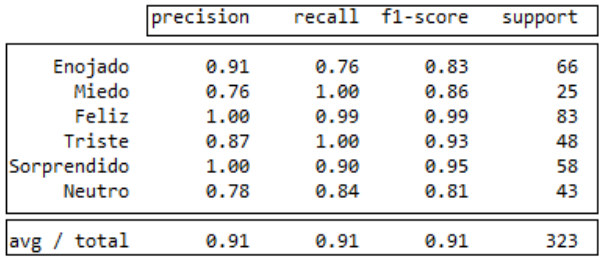
\includegraphics[width=100mm]{Imagenes/tabla_resultados_ck+.png} 
    \caption{Resultados obtenidos - CK+}
    \label{tab:tabla_resultados_ck+}
\end{table}

La tabla~\ref{tab:tabla_resultados_ck+} muestra los resultados obtenidos durante los experimentos realizados en la base de datos CK+. Dentro de los niveles de precisión y \textit{recall}, se observa que las categorías 'feliz' y 'sorpresa' obtienen mejores resultados que las demas (de igual forma que los resultados en la anterior base de datos), alcanzando un nivel de precisión de 100\% y 100\% respectivamente. Por otro lado, la categoría 'miedo' alcanza 46\%, siendo la mas baja de entre todas. El resultado general alcanzado en este conjunto de datos es de 91\%.

\begin{figure}[H]
		\centering
		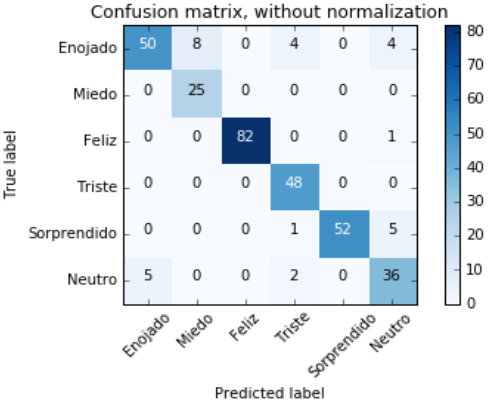
\includegraphics[width=90mm]{Imagenes/matriz_confusion_ck+.png}
		\caption{Matriz de confusión, precisión del Test - CK+}
		\label{fig:matriz_confusion_ck+}
\end{figure}

La figura~\ref{fig:matriz_confusion_ck+} muestra la matriz de confusión correspondiente a los resultados obtenidos para esta base de datos. Como se mostró en la tabla anterior, se puede observar que de las 82 muestras de la categoría 'feliz', todas son acertadas, alcanzando así el 100\% de precisión mencionado anteriormente. También se puede observar que en la categoría 'miedo' de las 88 imágenes en total, confunde 8 de ellas con la categoría 'enojado'. Otra de las categorías que también es confundida con las demás, es 'neutro', donde de 46 imágenes en total, 5 son confundidas con 'sorpresa', 4 con 'enojo' y 1 con 'feliz'.
 
\begin{figure}[H]
		\centering
		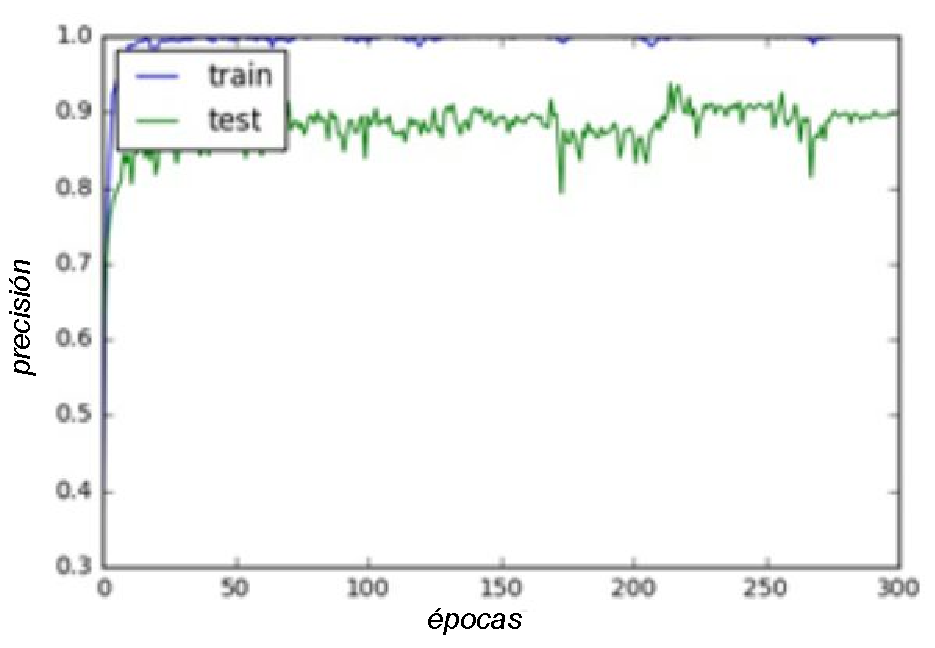
\includegraphics[width=95mm]{Imagenes/precision_ck+.pdf}
		\caption{Precisión durante el proceso de entrenamiento y prueba (\%) - CK+}
		\label{fig:precision-ck+}
\end{figure}

La figura~\ref{fig:precision-ck+} muestra la precisión alcanzada por la red durante el proceso de entrenamiento y pruebas en el transcurso de cada época. La linea azul representa la precisión alcanzada con los datos de entrenamiento, donde se observa claramente que este alcanza el 100\% de precisión aproximadamente en la época 50, sim embargo, también esta curva presenta oscilaciones en ciertas épocas, bajando ligeramente su nivel de precisión. La linea verde representa la precisión alcanzada con el conjunto de pruebas, el cual muestra el pico más alto de la curva entre la época 200 y 300, siendo este número de épocas el apropiado para obtener la mejor precisión posible.

\subsection{FER2013 - CK+}

\begin{table}[H]
    \centering
    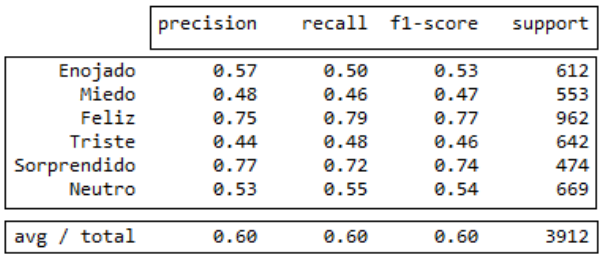
\includegraphics[width=100mm]{Imagenes/tabla_resultados_fer_ck+.png} 
    \caption{Resultados obtenidos - FER2013 - CK+}
    \label{tab:tabla_resultados_fer_ck+}
\end{table}

La tabla~\ref{tab:tabla_resultados_fer_ck+} muestra los resultados obtenidos durante los experimentos realizados en la unión de las bases de datos FER2013 y CK+. Dentro de los niveles de precisión y \textit{recall}, se observa que las categorías 'feliz' y 'sorpresa' obtienen mejores resultados que las demás (de igual forma que en las anteriores bases de datos), alcanzando un nivel de precisión de 75\% y 77\% respectivamente. Por otro lado, la categoría 'triste' alcanza 44\%, siendo la mas baja de entre todas. El resultado general alcanzado en este conjunto de datos es de 60\%.

\begin{figure}[H]
		\centering
		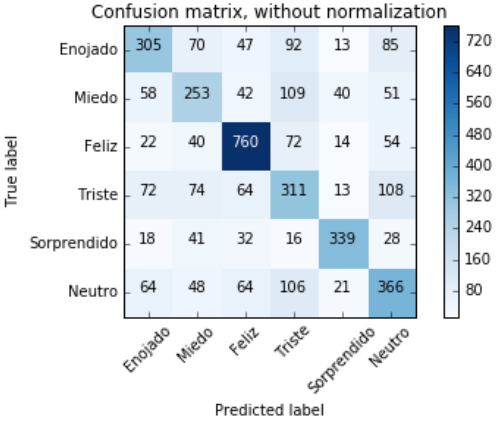
\includegraphics[width=90mm]{Imagenes/matriz_confusion_fer_ck+.png}
		\caption{Matriz de confusión, precisión del Test FER2013 - CK+}
		\label{fig:matriz_confusion_fer_ck+}
\end{figure}

La figura~\ref{fig:matriz_confusion_fer_ck+} muestra la matriz de confusión correspondiente a la unión de las dos bases de datos antes mencionadas. En ella se puede observar que muchas categorías son confundidas por las otras en cantidades considerables, sin embargo la categoría 'triste' es la que más errores comete, siendo 109 y 106 imágenes confundidas con la categorías 'miedo' y 'neutro' respectivamente. 
  
\begin{figure}[H]
		\centering
		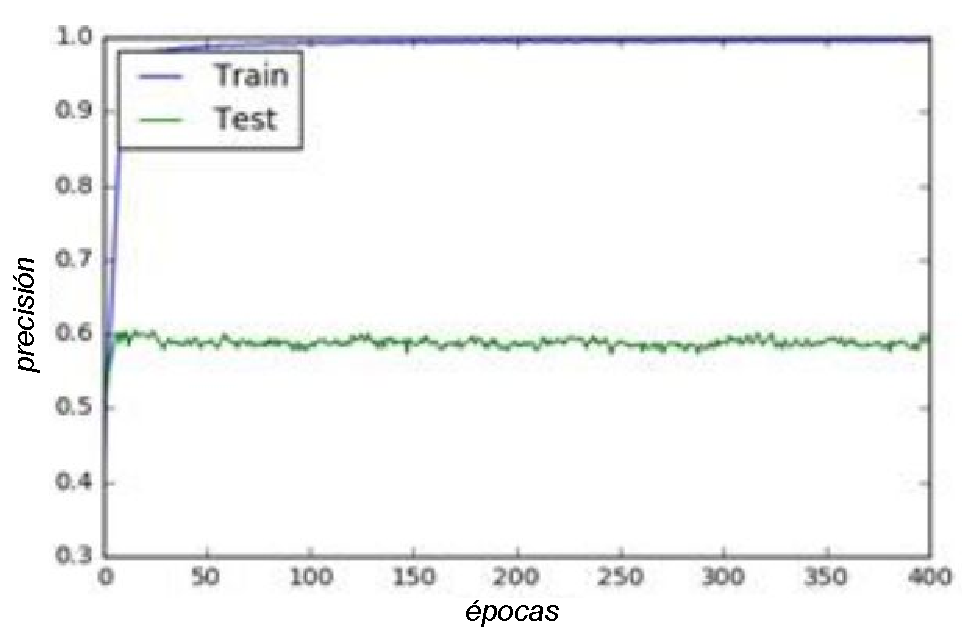
\includegraphics[width=95mm]{Imagenes/precision_fer_ck+.pdf}
		\caption{Precisión durante el proceso de entrenamiento y prueba (\%) FER2013 - CK+}
		\label{fig:precision_fer_ck+}
\end{figure}

En la figura~\ref{fig:precision_fer_ck+}, similar que en las dos anteriores gráficas de precisión correspondientes a las anteriores bases de datos, se puede observar que con los datos de entrenamiento se obtiene un nivel de precisión del 100\$, sin embargo, con los datos de entrenamiento se genera una curva con pequeñas oscilaciones durante el transcurso de las épocas, por lo tanto se concluye que utilizando un número de épocas mayor o igual a 20 se obtendra el máximo nivel de precisión.



